\section{Approximations for the Transparent Boundary Conditions for the dispersion equation}
\label{sec:approxTBC}

\indent The computation of the TBCs \eqref{eq:continuousTBC} is not simple due to the inverse Laplace transform that, which makes these conditions to be nonlocal in time. Therefore, we will propose approximations of the root \eqref{eq:lambda} that avoid integrations in time, making the TBCs considerably simpler.

\indent Obviously, as we can see through the results shown in this section, the approximate boundary conditions are not so precise as the ones proposed by \cite{besse2015} (who derives TBCs derived for the discrete linearized KdV equation). Nevertheless, the objectives of our work and the work of \cite{besse2015} are very different : while they seek to minimize the error of the computed solution (compared to the analytical one) due to the boundary conditions, we want here to apply our approximate TBCs as Coupling Boundary Conditions (CBCs) in a Domain Decomposition Method (DDM). Therefore, our objective lays on the convergence of the DDM to the solution of the same problem in the monodomain, independetly of the errors on the external boundaries. 

\indent For deriving our approximations, we firstly notice that we can rewrite \eqref{eq:continuousTBC} as

\begin{gather}
\label{eq:TBCnoConvolution}
    \begin{cases}
        u(t,a) - \laplinv \left( \frac{\lambda_1(s)^2}{s} \hat{u}_x(t,s) \right)  - \laplinv \left( \frac{\lambda_1(s)}{s}  \hat{u}_{xx}(t,s) \right) = 0 \\
        u(t,b) - \laplinv \left( \frac{1}{\lambda_1(s)^2}   \hat{u}_{xx}(t,s) \right) = 0 \\
        u_x(t,b) - \laplinv \left( \frac{1}{\lambda_1(s)}   \hat{u}_{xx}(t,s) \right) = 0 
    \end{cases}
\end{gather}

\noindent where $\hat{u}(s,x) = \mathcal{L}u(t,x)$ is the Laplace transform in $t$ of $u$.  Moreover, the inverse Laplace transform satisfies the following properties \cite{laplaceTransform}:

\begin{itemize}
	\item Linearity :
		\begin{equation}
			\label{eq:linearityLaplace}
				\laplinv \left[a_1\hat{u}_1(s,x) + a_2\hat{u}_2(s,x)\right] = a_1u_1(t,x) + a_2u_2(t,x)
		\end{equation}
	\item First Derivative : 
		\begin{equation}
			\label{eq:firstDerivativeLaplace}
			\laplinv \left[ s\hat{u}(s,x) \right] = u_t(t,x) + \laplinv \left[ u(0,x) \right] =  u_t(s,t) +  u(0,x) \delta (t)
		\end{equation}
	\item Second Derivative : 
		\begin{equation}
			\label{eq:secondDerivativeLaplace}
			\begin{aligned}
			\laplinv \left[ s^2\hat{u}(s,x) \right] = & u_{tt}(t,x) + \laplinv \left[ su(0,x) + u_{t}(0,x)\right] = \\
																		   & u_{tt}(s,t) + u(0,x)\delta_t(t) +  u_t(0,x)\delta (t)
			\end{aligned}
		\end{equation}
	\item Convolution :
	\begin{equation}
		\label{eq:convolutionLaplace}
		\laplinv \left[ \hat{u}_1(s,x)\hat{u}_2(s,x)\right] = \laplinv \left[ \hat{u}_1(s,x)\right] * \laplinv \left[ \hat{u}_2(s,x)\right]
	\end{equation}
\end{itemize} 

\noindent where $\delta (t)$ is the Dirac delta function and $*$ denotes the convolution operator.

\indent The properties \eqref{eq:linearityLaplace} to \eqref{eq:convolutionLaplace} motivate us to approximate the operands of the inverse Laplace transforms in \eqref{eq:continuousTBC} by polynomials in $s$. We will initially use a constant polynomial for this approximation. Before that, we remark the following useful relations between the mentioned operands, as a consequence of \eqref{eq:lambda}.

\subsection{Approximation of the TBCs using a constant polynomial}

\indent We will use the constant polynomial $P_0(s) = c$ for approximating $\frac{\lambda^2}{s}$. Moreover, as a consequence of \eqref{eq:lambda}, we can approximate the other operands of the inverse Laplace transforms in \eqref{eq:continuousTBC} only in function of $c$ :

\begin{equation}
	\label{eq:appP0}
	\frac{\lambda^2}{s}  = c \qquad
	\frac{\lambda}{s}  = -c^2 \qquad
	\frac{1}{\lambda_1(s)^2}  = c^2\qquad 
	 \frac{1}{\lambda_1(s)}  = -c 
\end{equation}

\indent Replacing \eqref{eq:appP0} in \eqref{eq:continuousTBC} and considering possibly different polynomial approximations for the left and the right boundaries (respectively with the coefficients $c_L$ and $c_R$), we get the approximate Transparent Boundary Conditions : 

\begin{equation}
\label{eq:appTBCP0}
    \begin{cases}
        u(t,a) - c u_x(t,a)  + c^2  u_{xx}(t,x) = 0 \\
        u(t,b) - c^2    u_{xx}(t,x) = 0 \\
        u_x(t,b) + c u_{xx}(t,x)= 0 
    \end{cases}
\end{equation}

\indent Considering a discrete domain with mesh size $\Delta x$ and points $x_0, ..., x_N$ and using some finite difference approximations, the approximate TBCs (\ref{eq:appTBCP0}) are discretized as

\begin{equation}
\label{eq:appDiscTBCP0}
    \begin{cases}
        u_0 - c_L \frac{u_1 - u_0}{\Delta x}  + c_L^2  \frac{u_0 -2u_1 + u_2}{\Delta x^2} = 0 \\
        u_N - c_R^2    \frac{u_N -2u_{N-1} + u_{N-2}}{\Delta x^2} = 0 \\
        \frac{u_N - u_{N-1}}{\Delta x}  + c_R^2    \frac{u_N -2u_{N-1} + u_{N-2}}{\Delta x^2} = 0 
    \end{cases}
\end{equation}

\subsubsection{Initial numerical experiments}

\indent In order to validate our approximation, observe its general behavior when varying the constant approximations $c_L$ and $c_R$ and compare our results with the ones obtained by \cite{besse2015}, we will solve the same numerical test presented in this paper. This problem,  originally treated by \cite{zheng2008} for the study of numerical solutions for the KdV equation, reads

\begin{gather}
\label{eq:testCaseBesse1}
 u_t + u_{xxx} = 0, \ \ x \in \mathbb{R} \\
 \label{eq:testCaseBesse2}
 u(0,x) = e^{-x^2}, \ \ x \in \mathbb{R}  \\
 \label{eq:testCaseBesse3}
 u \rightarrow 0, \ \ |x| \rightarrow \infty
\end{gather}

\indent The fundamental solution of (\ref{eq:testCaseBesse1}) and  the exact solution for the problem (\ref{eq:testCaseBesse1}) - (\ref{eq:testCaseBesse3}) are, respectively, 

\begin{equation}
    E(t,x) = \frac{1}{\sqrt[3]{3t}}Ai\left(\frac{x}{\sqrt[3]{3t}} \right)
\end{equation}

\begin{equation}
	\label{eq:exactSolution}
    u_{exact}(t,x) = E(t,x) * e^{-x^2}
\end{equation}

\noindent where $Ai$ is the Airy function.

\indent As done by \cite{zheng2008} and \cite{besse2015}, the problem will be solved in the spatial domain $[-6,-6]$, for $0 \leq t \leq T_{max}$, with $T_{max} = 4$. The mesh size is $\Delta x = 12/500 = 0.024$ and, as in \cite{besse2015}, the time step is $\Delta t = 4/2560 = 0.0015625$.

\indent For a quantitative evaluation of the results, we will calculate the same errors defined in the paper of \cite{besse2015}. For each instant $t_n = n\Delta t$, we compute the relative $l^2-$error

$$e^n = \frac{\left\Vert u_{exact}^n - u_{computed}^n\right\Vert_2}{\left\Vert u_{exact}^n\right\Vert_2}$$

\noindent and, in the whole time interval, the maximum error $e^n$ and the $l^2$ norm of $e^n$, given respectively by :

$$ e_{Tm} = \max\limits_{0 < n < T_{max}} (e^n) $$

$$ e_{L2} = \sqrt{ \Delta t \sum_{n=1}^{T_{max}} (e^n)^2 } $$

\indent In order to verify the influence of $c_L$ and $c_R$ on the computed solutions (and possibly identify a range of values that better approximate the TBCs), we made several tests with all the possible pairs $c_L,c_R \in \{-10,-1,-0.1,0,0.1,1,10\}^2$. The results were classified accordingly to their errors $e_{L2}$ (a criteria based on the error $e_{Tm}$ gives a similar result). The figure \ref{fig:firstTestsP0} shows, for some instants, a comparison between the best, the worst and the exact solution. For naming the worst result, we did not consider the ones in which the numerical solution diverged (following the arbitrary criteria $e_{L2} > 10$). 

\begingroup
\begin{minipage}{.5\linewidth}
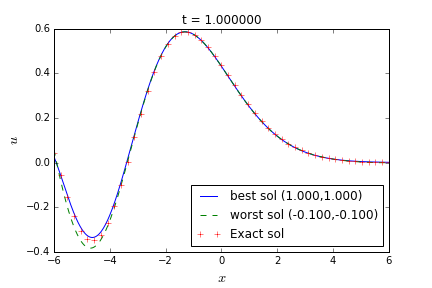
\includegraphics[scale=.5]{figures/BessefirstTestsP0Snap2.png}
\end{minipage}
\begin{minipage}{.5\linewidth}
	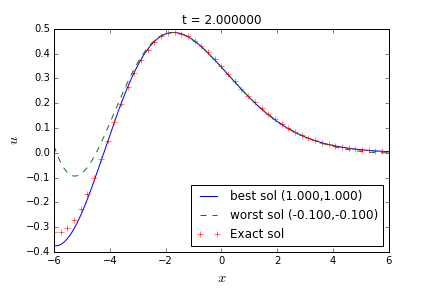
\includegraphics[scale=.5]{figures/BessefirstTestsP0Snap3.png}
\end{minipage}
\begin{minipage}{.5\linewidth}
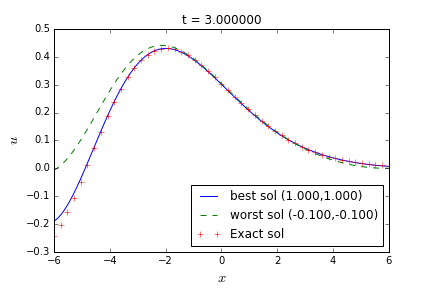
\includegraphics[scale=.5]{figures/BessefirstTestsP0Snap4.png}
\end{minipage}
\begin{minipage}{.5\linewidth}
	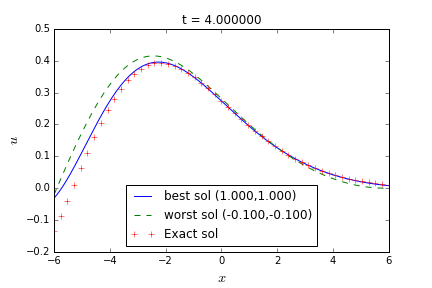
\includegraphics[scale=.5]{figures/BessefirstTestsP0Snap5.png}
\end{minipage}
\captionof{figure}{Best and worst solution compared with analytical solution, for the constant polynomial approximation \label{fig:firstTestsP0}}
\endgroup

\indent The table \ref{tab:firstTestsP0} presents the ten tests that presented the smallest $e_{L2}$ :

\sisetup{round-mode=places}
\begin{center}
\begin{tabular}{c|c|S[round-precision=4,table-number-alignment =  left]}
	\multicolumn{1}{c|}{$c_L$}  & \multicolumn{1}{c|}{$c_R$} & \multicolumn{1}{r}{$e_{L2}$} \\
	\hline
	1.0 & 1.0 & 0.0946839239675 \\
	1.0 & 10.0 & 0.097288371204 \\
	1.0 & 0.1 & 0.0983932287563 \\
	1.0 & 0.0 & 0.0992063806502 \\
	1.0 & -10.0 & 0.099359192771 \\
	1.0 & -0.1 & 0.100021589665 \\
	1.0 &  -1. & 0.10159265619 \\
	10.0 & 1.0 & 0.347003021321 \\
	10.0 & 0.1 & 0.347379492262 \\
	10.0 & 0.0 & 0.347487945035
\end{tabular}
\captionof{table}{Best results (smallest $e_{L2}$) for the constant polynomial approximation \label{tab:firstTestsP0}}
\end{center}

\indent We notice that the results are much sensitive to the coefficient on the left boundary : for a fixed $c_L$, the error is very similar for every $c_R$. This is a consequence of the fact that the solution of this specific problem is practically constant and equal to zero near $x = 6$, but presents strong variations in time near $x = -6$. The best result, as shown in the figure \ref{fig:firstTestsP0}, is able to impose this condition on the right boundary, what the worst solution is not able to do. In the case of the left boundary, in despite of a more evident error, the best solutions follows quite well the behavior of the exact solution.

\subsection{Approximation of the TBCs using a linear polynomial}

\indent In a similar way as done above, we approximate  $\frac{\lambda^2}{s}$ by $P_1(s) = ds + c$. Then, using relations similar to \eqref{eq:appP0}, the inverse Laplace transforms in \eqref{eq:TBCnoConvolution} reads :

\begin{equation*}
	\begin{aligned}
    \mathcal{L}^{-1} \left( \frac{\lambda^2}{s} \hat{u}_x(s,x) \right) = & \mathcal{L}^{-1} \left[ (ds+c) \hat{u}_x(t,s) \right] = \\
    			 & d\mathcal{L}^{-1} \left[ \hat{u}_{xt}(t,s) \right] + c \mathcal{L}^{-1} \left[ \hat{u}_{x}(t,s) \right] = \\
    			 &   du_{xt}(x,t) + du_x(0,x)\delta (t) + cu_x(x,t) \\
    \mathcal{L}^{-1} \left( \frac{\lambda}{s} \hat{u}_{xx}(s,x) \right) = & \mathcal{L}^{-1} \left[ -(ds+c)^2 \hat{u}_{xx}(t,s) \right] =\\
    			&  -d^2u_{xxtt}(x,t) - d^2\delta_t(t) u_xx(0,x) - d^2 \delta(t)u_{xxt}(0,x)  + \\ 
    			& - 2dcu_{xxt}(x,t) -  2dcu_xx(0,x)\delta (t) - c^2u_{xx}(x,t) \\
    \mathcal{L}^{-1} \left( \frac{1}{\lambda^2} \hat{u}_{xx}(s,x) \right) = & \mathcal{L}^{-1} \left[ (ds+c)^2 \hat{u}_{xx}(t,s) \right] = \\
    			& d^2u_{xxtt}(x,t) + d^2\delta_t(t) u_xx(0,x) + d^2 \delta(t)u_{xxt}(0,x)  + \\
    			& 2dcu_{xxt}(x,t) +  2dcu_xx(0,x)\delta (t) + c^2u_{xx}(x,t) \\
    \mathcal{L}^{-1} \left( \frac{1}{\lambda} \hat{u}_{xx}(s,x) \right) = & \mathcal{L}^{-1} \left[ -(ds+c) \hat{u}_{xx}(t,s) \right] = \\
    			& -du_{xxt}(x,t) - du_{xx}(0,x)\delta (t) - cu_{xx}(x,t)
\end{aligned}
\end{equation*}

\indent Using forward first order forward finite difference approximations for the first derivative in time, second order centered for the second derivative in time, and considering that the initial solution and its derivatives are equal to zero on the boundaries (which is the case of the test case treated here), we obtain the following discretized approximate TBCs : 

\begin{equation*}
\label{eq:appDiscTBCP1}
	\begin{aligned}
    u_0^{n+1} - \left( \frac{d_L}{\Delta t} + c_L \right) \left( \frac{u_1^{n+1} - u_0^{n+1}}{\Delta x}\right) +   \left( \frac{d_L^2}{\Delta t^2} + \frac{2d_Lc_L}{\Delta t} + c_L^2  \right) \left(  \frac{u_0^{n+1} - 2u_1^{n+1} + u_2^{n+1}}{\Delta x^2} \right)  = \\
        -\frac{d_L}{\Delta t}\left( \frac{u_1^{n} - u_0^{n}}{\Delta x}\right) +  \left( 2\frac{d_L^2}{\Delta t^2} + \frac{2d_Lc_L}{\Delta t}\right) \left(  \frac{u_0^{n} - 2u_1^n + u_2^{n}}{\Delta x^2} \right)    -  \frac{d_L^2}{\Delta t^2} \left(  \frac{u_0^{n-1} - 2u_1^{n-1} + u_2^{n-1}}{\Delta x^2} \right)
   \end{aligned}
\end{equation*} 

\begin{equation*}
	\begin{aligned}
    u_N^{n+1} - \left( \frac{d_R^2}{\Delta t^2} + \frac{2d_Rc_R}{\Delta t} + c_R^2  \right) \left(  \frac{u_{N}^{n+1} - 2u_{N-1}^{n+1} + u_{N-2}^{n+1}}{\Delta x^2} \right) = \\
     -\left( 2\frac{d_R^2}{\Delta t^2} + \frac{2d_Rc_R}{\Delta t}\right) \left(  \frac{u_N^{n} - 2u_{N-1}^n + u_{N-2}^{n}}{\Delta x^2} \right) + \frac{d_R^2}{\Delta t^2} \left(  \frac{u_N^{n-1} - 2u_{N-1}^{n-1} + u_{N-2}^{n-1}}{\Delta x^2} \right)
    \end{aligned}
\end{equation*} 
   
\begin{equation*}
	\begin{aligned}	
    \frac{u_N^{n+1} - u_{N-1}^{n+1}}{\Delta x} + \left( \frac{d_R}{\Delta t} + c_R \right) \left( \frac{u_N^{n+1} -2 u_{N-1}^{n+1} + u_{N-2}^{n+1}}{\Delta x^2}\right) =      \frac{d_R}{\Delta t}\left( \frac{u_{N}^{n} - 2u_{N-1}^{n} + u_{N-2}^n}{\Delta x^2}\right)
    \end{aligned}
\end{equation*}

\subsubsection{Initial numerical experiments}

\indent We repeated the numerical tests made for the approximation with $P_0$, making the coefficients $c_L$ and $d_L$ assume the values in $\{-10,-1,-0.1,0,0.1,1,10\}$. In order to avoid a too high computation, and also taking in account the remark we made above about the weak dependence of the results on the coefficients for the right boundary, all the tests were done assuming $c_R = c_L$ and $d_R = d_L$.

\indent We present in the table \ref{tab:firstTestsP1} the ten best results. As we can see, the best result is the one where $d_L = d_R = 0$ and $c_L = c_R = 1. $, which corresponds to the best results of the approximations using constant polynomials.

	 \sisetup{round-mode=places}
\begin{center}
\begin{tabular}{c|c|S[round-precision=4,table-number-alignment =  left]}
	\multicolumn{1}{c|}{$d_L = d_R$}  & \multicolumn{1}{c|}{$c_L = c_R$} & \multicolumn{1}{r}{$e_{L2}$} \\
	\hline
	0. & 1.0 & 0.0946839239675 \\
	0.1 & 1.0 & 0.12341195 \\
	1.0 & 1.0 & 0.20031603 \\
	10.0 & 0.1 & 0.22037249 \\
	-10.0 & 0.1 & 0.23984486 \\
	10.0 & 1.0 & 0.27161158 \\
	-10.0 &  0.0 & 0.24800816\\
	-10.0 & 1.0 & 0.30039637 \\
	10.0 & 0.0 & 0.27213611 \\
	0.0 & 0.1 & 0.36740764
\end{tabular}
\captionof{table}{Best results (smallest $e_{L2}$) for the linear polynomial approximation \label{tab:firstTestsP1}}
\end{center}

\subsection{Partial conclusion}

\indent It must be clear that our approach is not better than the one proposed by \cite{besse2015}, what, as discussed in the section \ref{sec:errors} of this paper, it is not the objective of the work developed here. Indeed, \cite{besse2015} derives TBCs for two discrete schemes, and the worst result among them, using the same $\Delta x $ and $\Delta t$ that we used here, presents an error $e_{L2} \approx 0.005$ for $t = 4$, while our best result has $e_{L2} \approx 0.1$ for the same instant.

\indent However, we can say that the boundary conditions proposed here work relatively well as TBCs, with a very simple implementation and, consequently, low computation and memory costs. Moreover, as shown in the results of this section, the approximation using a linear polynomial, although the increment in the complexity (including time derivative terms up to the second derivative, what requires the storage of previous computed solutions), does not provide a better approximation for the TBC, in comparison with the approximation using a constant polynomial. Therefore, in the following, we will use only this last approximation, for which the TBCs will be denoted as  

\begin{equation*}
    \begin{gathered}
        \Theta_1^{c_L}(u,x) = u(t,x) - c_L u_x(t,x)  + c_L^2  u_{xx}(t,x) \\
        \Theta_2^{c_R}(u,x) =  u(t,x) - c_R^2    u_{xx}(t,x)\\
        \Theta_3^{c_R} (u,x)= u_x(t,x) + c_R u_{xx}(t,x) 
    \end{gathered}
\end{equation*}

\subsection{Optimization of the approximate TBCs (minimization of the errors compared to the analytical solution)}

\indent In this subsection, we investigate deeply the influence of the constant polynomial approximation over the error of the computed solution, compared with the analytical one. For this purpose, we repeat the computations, but with a much more refined range of coefficients, always using as criteria of quality the error $e_{L2}$ of each test.

\indent As a consequence of the remarks made in the last subsection, this refinement is made higher for the coefficient $c_L$. By making a gradual study, in which we identified at each step the intervals of $c_L$ which give the best results and studied it even more deeply (up to a step $0.01$ for the variation of $c_L$), we were able to construct the curves presented in the figure \ref{fig:optimTBC} and identify the empirical optimum $c_L = 1.16$ :

\begingroup
\begin{minipage}{.5\linewidth}
	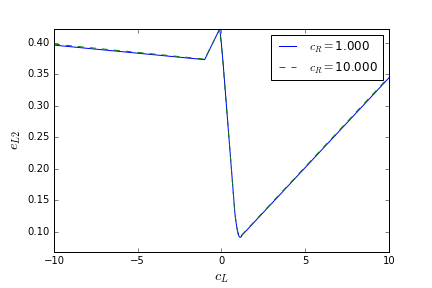
\includegraphics[scale=.45]{figures/errorOptimOnlyL2.png}
	\captionof{subfigure}{General view of all the tested coefficients}
\end{minipage}
\begin{minipage}{.5\linewidth}
	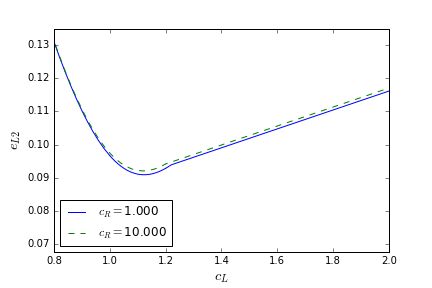
\includegraphics[scale=.45]{figures/errorOptimOnlyL2Detail.png}
	\captionof{subfigure}{Detail for $c_L \in [0.8,2.0]$}
\end{minipage}
	\captionof{figure}{Error of the numerical solution compared to the analytical solution as function of the constant polynomial approximation for the TBC \label{fig:optimTBC}}
\endgroup